\documentclass[11pt]{scrartcl}
\usepackage[sexy]{../evan}
\usepackage{cmbright}
\usepackage{cancel}
\usepackage[T1]{fontenc}
%\usepackage{enumerate}
\usepackage[shortlabels]{enumitem}
\usepackage[utf8]{inputenc}
\usepackage[margin=1in]{geometry}
%\usepackage[pdfborder={0 0 0},colorlinks=true,citecolor=red{}]{hyperref}
\usepackage{amsmath}
\usepackage{amssymb}
\usepackage{setspace}
\usepackage{systeme}
%\usepackage[vlined]{algorithm2e}
\usepackage[linesnumbered,ruled,vlined]{algorithm2e}
\usepackage{mathtools}
\usepackage{graphicx}
\graphicspath{ {./images/} }
\SetStartEndCondition{ }{}{}%
\SetKwProg{Fn}{def}{\string:}{}
\SetKwFunction{Range}{range}%%
\SetKw{KwTo}{in}\SetKwFor{For}{for}{\string:}{}%
\SetKwIF{If}{ElseIf}{Else}{if}{:}{elif}{else:}{}%
\SetKwFor{While}{while}{:}{fintq}%
\newcommand{\forcond}{$i=0$ \KwTo $n$}
\SetKwFunction{FRecurs}{FnRecursive}%
\AlgoDontDisplayBlockMarkers\SetAlgoNoEnd\SetAlgoNoLine%


\usepackage{xcolor}
\DontPrintSemicolon

% Define pseudocode formatting
\renewcommand{\KwSty}[1]{\textnormal{\textcolor{blue!90!black}{\ttfamily\bfseries #1}}\unskip}
\renewcommand{\ArgSty}[1]{\textnormal{\ttfamily #1}\unskip}
\SetKwComment{Comment}{\color{green!50!black}// }{}
\renewcommand{\CommentSty}[1]{\textnormal{\ttfamily\color{green!50!black}#1}\unskip}
\newcommand{\assign}{\leftarrow}
\newcommand{\var}{\texttt}
\newcommand{\FuncCall}[2]{\texttt{\bfseries #1(#2)}}
\SetKwProg{Function}{function}{}{}
\renewcommand{\ProgSty}[1]{\texttt{\bfseries #1}}



\title{CS 577: Final}
\author{Daniel Ko}
\date{Summer 2020}

\begin{document}
\maketitle


\section{
  A sawmill only has one large sawing machine and get $n$ job orders at the
  beginning of each day. They want the jobs to be scheduled in an order that keeps the customers
  most satisfied
 }
\subsection{
	Someone proposes to schedule the jobs based on the descending order of the
	value of the corresponding customers. That is, the one with the highest value get the job
	scheduled first. In the above example, the customer with value 20 is scheduled before the
	customer with the value of 2. Show a counter example that this greedy algorithm will not
	result in the lowest average valued finishing time.
}
Consider the two following jobs, $v_\alpha = 10, t_\alpha =1$ and  $v_\phi = 5, t_\phi =0.1$
The lowest average valued finishing time using the greedy algorithm will result in,
$$
	\frac{1}{2}\Big( (10)(1) + (5)(1.1) \Big) = 7.75
$$
However, if we switch the scheduling, we can observe a lower overall average,
$$
	\frac{1}{2}\Big( (5)(0.1) + (10)(1.1) \Big) = 5.75
$$
Hence, this greedy solution is not optimal.

\subsection{
	Design an optimal greedy algorithm to solve the problem and analyze the
	computing complexity. Here you just need to state the algorithm idea but do not have to
	write out the pseudocode.
}

Consider the algorithm where we schedule the jobs based on the descending order
of the ratio of value to time, i.e. $v_\alpha / t_\alpha$.
The computing complexity for this algorithm will be the time it takes to compute these ratios, $n$ time,
and to sort these ratios which will take $n \log n$ time if we use a fast sorting algorithm like merge sort.
Hence our total computing complexity will be $O(n + n \log n) = O(n \log n)$.

\subsection{
	Prove the optimality of your algorithm using either “Exchange argument” or
	“Stay ahead” method.
}
We show by exchange argument that our algorithm is optimal.
\subsubsection{
	Define the solution
}
Let $O =\{o_1, \cdots, o_n \}$ be the order in which the optimal solution orders the jobs.
Let $A =\{a_1, \cdots, a_n \}$ be the order in which the my solution orders the jobs.
\subsubsection{
	Identify the difference
}
If $O \neq A$, there must exist adjacent jobs $\alpha$ and $\phi$ such that job $\alpha$ is scheduled earlier than job $\phi$
in the optimal solution and job $\phi$ is scheduled earlier than job $\alpha$ in the greedy solution.
\subsubsection{
	Exchange and iterate
}
For our greedy algorithm we know that, $v_\phi / t_\phi \geq v_\alpha / t_\alpha$ because we scheduled the jobs in this way.
Let $\delta$ denote the finish time before jobs $\alpha$ and $\phi$ in the optimal solution.
In the original order, the weights of these two jobs in the optimal solution are
$$v_\alpha (\delta + t_\alpha) +  v_\phi (\delta +  t_\alpha + t_\phi)$$
If we swap to our greedy solution, the weights of these two jobs are
$$v_\phi (\delta + t_\phi) +  v_\alpha (\delta +  t_\phi + t_\alpha)$$
If we take the difference between the greedy and optimal weights and using the fact that $v_\phi / t_\phi \geq v_\alpha / t_\alpha$, we get
$$v_\alpha t_\phi - v_\phi t_\alpha  \leq 0$$
This means that swapping $\phi$ and $\alpha$ in the optimal solution to the order of the greedy solution
does not increase the completion time, meaning this swapped 
order is optimal as well. We can swap all such jobs without increasing the completion time, and at the end of this 
processes we will have job ordering identical to our greedy algorithm. Therefore, the job order produced by our algorithm must 
be optimal. 
\pagebreak

%%%%%%%%%%%%%%%%%%%%%%%%%%%% NETWORK FLOW %%%%%%%%%%%%%%%%%%%%%%%%%%%%%%%%%%%%%%%%
%file:///C:/Users/Daniel/Downloads/CS577Summer20Assignment6Answer.pdf
%\begin{commentout}

	\section{
	  Which of the remaining applications should be migrated? Give a polynomial-time
	  algorithm to find a set $S \subseteq \{1, 2, \cdots , n-1\}$ for which the sum of the benefits minus the
	  interaction expenses happened after migration of the applications in $S$ is maximized.
	 }

	\subsection{
		Construct a network flow model for this problem. Clearly state the meaning of
		each component (node, edge, capacity) of the flow network that you construct, set up a flow
		network graph, describe your algorithm idea (you don’t have to write the pseudocode), and
		give the computing complexity analysis of your algorithm
	}
	We construct a directed graph $G=(V,E)$ to model the network flow.
	\subsubsection{
		Components for graph
	}
	\begin{enumerate}[label=\alph*.]
		\item{
		      \textbf{Nodes}
		      \begin{itemize}
			      \item Start with a source node $s$.
			      \item Add a column of $n-1$ nodes, denoted as $a$, to represent the number of application.
			      \item Add node $a_n$ to represent application $n$. Let this be our sink node.
		      \end{itemize}
		      }
		\item{
		      \textbf{Edges and capacities}
		      \begin{itemize}
			      \item{
			            Add edges from source node $s$ to each application node $a_i$, excluding $a_n$. Let the capacity of these edges be $b_i$.
			            }
			      \item {
						Add edges from $a_i \rightarrow a_j$ and $a_j \rightarrow a_i$ with capacity $x_{ij}$ if such capacity is not zero and
						when $i \neq j$
			            }
		      \end{itemize}
		      }
	\end{enumerate}
	\begin{center}
		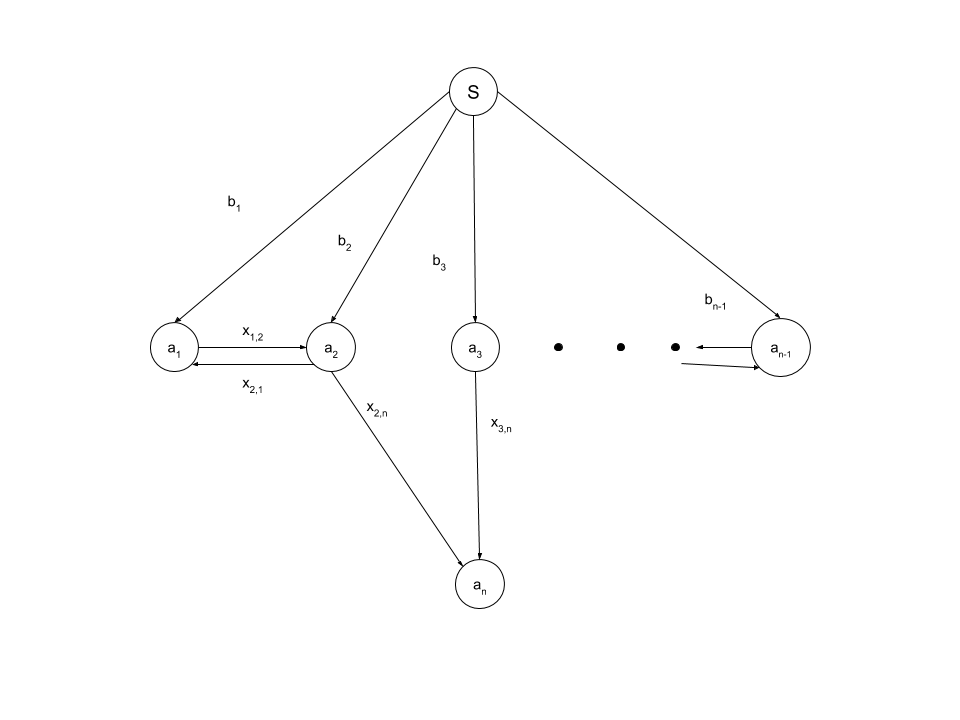
\includegraphics[scale=0.4]{final.png}
	\end{center}
	\subsubsection{
		Algorithm and complexity
	}
	The basic algorithm is to run Ford Fulkerson on our graph $G$ and return the set that contains the min-cut. 
	We want to compute set $M$, which contains the applications that will migrate, such that the net benefit 
	will be maximized, 
	$$ 
	\text{net benefit } = \sum_{v_i \notin M} b_i - \sum_{v_i \in M \land v_i \notin V \setminus M}  x_{ij}
	$$
	Using the min-cut max-flow theorem, we can compute the max flow to compute this value. 
	\begin{proof}
		The time complexity for setting up the graph is clearly $O(n^2)$.
		The time complexity for Ford Fulkerson is $O(\text{maxflow}|E|)$. The max number of edges we can have
		is $n + 2n^2$. The greatest max flow we can have is if there is no expense and we can move all 
		applications to the new sever, which would be $\sum b_i$. Hence, our time complexity would be 
		$O(n^2) + O((\sum b_i)(n + 2n^2)) = O(n^2\sum b_i)$.
	\end{proof}


	\pagebreak



%%%%%%%%%%%%%%%%%%%%%%%%%%%% NP PROBLEM %%%%%%%%%%%%%%%%%%%%%%%%%%%%%%%%%%%%%%%%
%\begin{commentout}

\section{
  Resource Allocation Problem
 }

\subsection{
	Prove that the Resource Allocation problem is an NP problem
}
%,and either if the set $S$ .  
\begin{proof}
	Suppose we have a set $S$ containing a list of $k$ applications claiming it satisfies the Resource Allocation problem.
	We can check if this set satisfies the Resource Allocation problem by iterating through each resource and check if 
	only one application requests it. We have an upper bound on the amount of resources that an application
	uses, which is $m$.  Hence, our computing complexity is $O(mkm) = O(km^2)$, which clearly takes polynomial time.
	Therefore, Resource Allocation is an NP problem.
\end{proof}


\subsection{
	Identify a well-known NP-Complete problem and show the construction of a
	Resource Allocation problem out of the well-known NP-Complete problem.
}
\begin{proof}
	We claim that we can reduce Resource Allocation problem to the Independent Set problem.
	We show that Independent Set $\leq_p$ Resource Allocation.

	Suppose we have a graph $G=(V,E)$, and we want to find an independent set of at least $k$.
	We can convert this problem into a Resource Allocation problem in polynomial time by doing the following.
	Create $|V|$ number of applications, each representing one vertex from our graph. 
	Create $|E|$ number of resource, each representing one edge from our graph. 
	For each application, assign the resources which corresponds to its edges in $G$. 
	
\end{proof}

\subsection{
	Show the correctness of the reduction.
}
\begin{proof}
	We claim that there is an independent set of size $k$ if and only if there are $k$ applications that are active. 

	If there is an independent set of size $k$, then its corresponding resources (which represent edges), will only be 
	assigned to at most one application. This means that all $k$ applications can be activated. 

	If there are $k$ applications that are active, this means that the corresponding vertices do not share any edges. 
	Hence, there exists an independent set of size $k$. 
\end{proof}

Thus, Independent Set $\leq_p$ Resource Allocation as desired.
Using Theorem 8.14, we conclude that Resource Allocation is NP-complete.

%\end{commentout}

\pagebreak

\section{Short answer questions}

\subsection{
	Maximum flow and minimum cut problem
}

\begin{enumerate}[label=\alph*.]
\item {
	32 is the max flow
}

\item{
	\-\\
	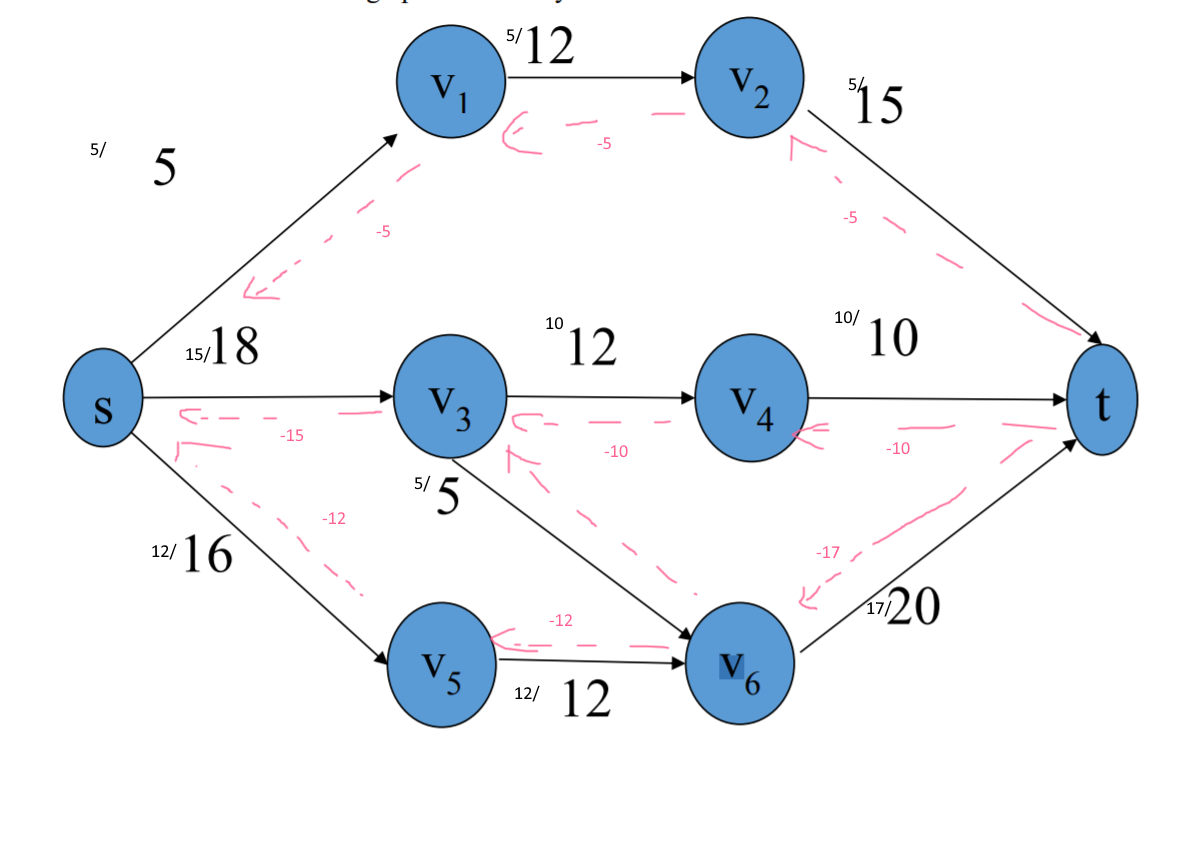
\includegraphics[scale=0.5]{graph4a}
}
\end{enumerate}

\subsection{
	True/False
}
\begin{enumerate}[label=\alph*.]
	\item {
		Yes, by cut property. 
	}
	
	\item{
	No. Consider the 2-Sat problem. We can trivally reduce it to 3-Sat, a NP complete problem, but we know 
	there exists a polynomial time algorithm for 2-Sat. See \url{https://en.wikipedia.org/wiki/2-satisfiability#Algorithms}
	}
\end{enumerate}
	


\end{document}

